% This is a template for  Masters' Theses at WPI.
% It complies (more or less) to the standards given by the Library 
% (as of February 1999)
%
% Feel free to use this file, but I give no guarantee for its compliance
% to standards (meaning I won't pay for the paper if the library rejects it :))
%
%
% The lengths (textheight, width etc.) are fine-tuned for ps1, ps2, and ps3, 
% but seem to be somewhat dependent on the machine you are using to compile, 
% the date, time, moon phase, the weather, and other quantum effects.
% You may have to change \oddsidemargin a little, but it's about 98% correct.
%
% Also, the spacing is correct (doublespacing with footnotes correctly
% singlespaced). Curiously, the font size is not specified in the
% regulations. So feel free to change it, but the majority of theses
% that I have seen is written in 12 point font.
% 
% As for the inclusion of graphics, I recommend the methods specified
% in ``latexguide.ps'' off the CS-GSO Website. You can use other
% methods including copy and paste with a photocopier, but I think
% using the graphicx package is the easiest.
%
% Have fun and good luck with the thesis.
%
%
%  Andreas Koeller (koeller@wpi.edu)
%
%
%

% The preamble
\documentclass[12pt]{report}
\def\algbackskip{\hskip-\ALG@thistlm}


% this enables correct linespacing and graphics inclusion via 
%``\includegraphics''
\usepackage{setspace}
\usepackage{graphicx}
\usepackage{float}
\usepackage{wrapfig}
\usepackage{acronym}
\restylefloat{figure}
\usepackage{cite}
\usepackage{gensymb}
\usepackage{url}
\usepackage{hyperref}
\usepackage[toc]{glossaries}
\usepackage{nomencl}
\makenomenclature
\usepackage[toc,page]{appendix}
\usepackage{caption}
\usepackage{amsmath} % Matrices
%\usepackage{subcaption}
\usepackage{pdflscape}
\usepackage{multirow}
\usepackage{multicol}
\usepackage[nottoc,numbib]{tocbibind}

\usepackage[noend]{algpseudocode}
\usepackage[margin=1.5in]{geometry}
\usepackage{amsfonts}
\usepackage{subcaption}
%\usepackage{subfloat}
\usepackage{epstopdf}
\usepackage[mathscr]{euscript}

%Code settings:
\usepackage{listings}
\usepackage{color}
\usepackage{pdfpages}
\usepackage{algorithm}
\usepackage{soul} %For highlighting, can remove later
% Fix quotes
\usepackage [english]{babel}
\usepackage [autostyle, english = american]{csquotes}
\MakeOuterQuote{"}
 
\lstdefinestyle{mystyle}{
    backgroundcolor=\color{backcolour},   
    commentstyle=\color{codegreen},
    keywordstyle=\color{magenta},
    numberstyle=\tiny\color{codegray},
    stringstyle=\color{codepurple},
    basicstyle=\tiny,
    breakatwhitespace=false,         
    breaklines=true,  
    frame=none,               
    captionpos=b,                    
    keepspaces=true,                 
    numbers=left,                    
    numbersep=5pt,                  
    showspaces=false,                
    showstringspaces=false,
    showtabs=false,
    framexleftmargin=5pt,                 
    tabsize=2
}
\lstset{style=mystyle}
%end code settings
\captionsetup[table]{skip=10pt}
% leave 1.5in margin to the left and 1in margin to the other
% sides. Don't print page number in the margin (but rather above it)
\setlength{\textheight}{8.63in}
\setlength{\textwidth}{5.9in}
\setlength{\topmargin}{-0.2in}
\setlength{\oddsidemargin}{0.3in}
\setlength{\evensidemargin}{0.3in}
\setlength{\headsep}{0.0in}

% Directory for images
\graphicspath{ {img/} }

\begin{document}
	% Define \brk as a command for leaving a little vertical space. Makes
	% the titlepage easier to read - normally, this is NOT GOOD LATEX
	% STYLE!!!
	\newcommand{\brk}{\vspace*{0.18in}}
	
	% No page number on the title page
	\thispagestyle{empty}
	
	% Center the whole title page
	\begin{center}
		
		\brk
		
		% Large font and bold face for the headline. Try to keep it at one or
		% two lines. Headlines over two lines will mess up the spacing, and you have to
		% manually finetune it. Note that the line break in the SOURCE CODE
		% does not affect the line breaking in the output file. If you want
		% hardcoded line breaks, you have to mark them with a double backslash (\\)
		
		{\large 
			\textbf{
				Extension on Adaptive MAC Protocol for Space Communications
			}
		}		
		
		\brk
		by
		
		\brk
		Max Li
		
		\brk
		\brk
		A Master's Thesis
		
		\brk
		Submitted to the Faculty 
		
		\brk
		of the
		
		\brk
		\brk
		WORCESTER POLYTECHNIC INSTITUTE
		
		\brk
		\brk
		In partial fulfillment of the requirements for the
		
		\brk
		Degree of Master of Science
		
		\brk
		in
		
		\brk
		Electrical and Computer Engineering
		
		\brk
		May 2018/Dec 2018s
	\end{center}
	
	% Remove paragraph indent temporarily
	\setlength{\parindent}{0pt}
	\brk
	\brk
	\brk
	APPROVED:\\

	\rule{3in}{0.8pt}\\
	Professor Alex Wyglinski, WPI ECE, Advisor\\

    \rule{3in}{0.8pt}\\
	Committee Member \#1\\

    \rule{3in}{0.8pt}\\
    Committee Member \#2\\

	\setlength{\parindent}{1.5em}

	% end of titlepage
	\newpage
	
	% This is the command for doublespacing when you use the setspace
	% package
	% Please do NOT use \baselinestretch, this will mess up everything,
	% cause earthquakes, tornados and lots of questions for me...
	% If you need a singlespaced paragraph (BAD STYLE!!!), use
	% \singlespacing or \onehalfspacing and enclose it together with the
	% paragraph in braces {\singlespacing This is my text... blah blah blah}
	%
	\doublespacing
	
	\begin{abstract}
		TODO. Secondary test edit to see if I can update git in both operating systems.
	\end{abstract}

	\pagenumbering{roman} % or {Roman} if you like them capitalized
	
	\chapter*{Acknowledgements}
	 TODO x 2
	\clearpage
	
	% Automagic
	\tableofcontents
	\listoffigures
	\listoftables
	

\chapter*{Acronyms}
A table of acronyms used in this report. Update with acronyms when used.
	\clearpage

	% And we need a clear separation between preface and text, otherwise
	% the numbering gets confused.
	\pagenumbering{arabic}
	\setcounter{page}{1}
	
    \chapter{Introduction}
\section{Motivation}
\par In recent times, the amount of computing power available has increased to the point where many techniques that have previously been considered too complex for certain time-sensitive applications have become feasible \cite{computationPower_ML}. The increase in computing power includes the general purpose processors (GPPs) that most people are familiar with, but also graphics processing units (GPUs) and field-programmable gate arrays (FPGAs), which are more suited to specialized applications. One field with potential to benefit from these developments is space communications, for which an increase in computing power enables the use of Software Defined Radios (SDRs)\cite{tim1, tim2}. SDRs provide flexibility by enabling many aspects of communications that are typically implemented in hardware to be implemented in software. This includes tasks such as such as filtering and detection of signals, as well as higher level things like reconfiguration of applications and services. \cite[p.~xxxiii]{SDRTextbook}. The idea of software implementation of hardware elements is not particularly new, but was previously difficult to implement with the computing power available. As the computing power at any given price point increased, cognitive communication algorithms that utilize the manuverability of SDRs were proposed. Many of the algorithms that have been implemented and tested focus on employing dynamic spectrum access techniques or other sensing approaches. In more recent times, many technologies have taken a different approach by attempting to achieve multi-objective goals through the modification of multiple radio parameters in a manner that rewards good behaviors. This learning behavior sets a foundation for the development of cognitive systems. This increased focus on multi-objective goals has been in part motivated by the satellite communications industry, which has proposed business ventures involving hundreds of spacecraft. With satellite communications, objectives have the potential to interact in complicated ways and may be inversely related in some cases. Maintaining "good" performance requires a balancing of these objectives. These large networks of satellites, combined with the recent interest in space exploration, motivate communication methods that have high link availability and robustness\cite{paulo6}. A cognitive communications system is likely necessary in acheiving both of these requirements satisfatorily, especially for situations where autonomous operation is required.

\par One of the more general purpose technologies that has experienced large growth from the boom in processing power is Artificial Intelligence (AI), or more specifically Machine Learning (ML). Breakthroughs like IBM's Watson \cite{watsonPaper} and DeepMind's AlphaGo\cite{paulo5} have been driven by the ability to use large amounts of computing power to apply increasingly more complex Deep Learning (DL) techniques, such as convolutional neural networks (CNNs) and deep-Q networks (DQNs)\cite{paulo5}. These techniques have typically involved too many computations to be considered tractible for many problems. However, the recent explosion of computing power available has enabled the use of these DL techniques that reach performance and speed thresholds previously thought impossible. This allows for a whole variety of new fields of application that may have stricter timing or accuracy requirements. 


\section{State of the Art}
\par In this section, an overview of recent developments in satellite communications and cognitive radio as they relate to this thesis will be provided. 
\subsection{Satellite Communications}
\par Within the field of satellite communications, the most relevent developments are in the fields of Adaptive Coding and Modulation (ACM) schemes and satellite transmission standards.  ACM is used in the situation that received signal power changes due to impairments in the channel\cite{acm_explained}. This change in power is often a result of fading, which can be caused by weather conditions or the relative motion between the transmitter and the receiver \cite{paulo17}, among other things. ACM adaptively chooses the modulation and coding scheme based on the observed link budget and the quality of the message at the receiver, usually by looking for the optimal configuration in a table. ACM has been applied to 
Geosynchronous Equatorial Orbit (GEO) satellite channels operating in the S-band \cite{paulo18} as well as the Ka-band \cite{paulo19}. In this work, it is considered to be the standard solution for Low Earth Orbit (LEO) satellite links.  
%\textit{No direct comparisons to ACM will be made, as ACM is used primarily in situations where changes in the channel are somewhat predictable \textbf{[confirm this]}}.
\par In the context of satellite communications, there are a number of different standards that can be used in transmission of data. For this thesis, DVB-S2 \cite{paulo21} was chosen as the standard that represents most modern satellites. This standard is the second generation of DVB-S, a technical standard for GEO satellite-based digital television brodcast systems that was primarily desigend for direct-to-home services. Most of the innovations of DVB-S2 are present in the physical (PHY) layer in the OSI model \cite{placeholderCitation}, with more e-client channel coding, modulation, and error correction techniques. In addition, it uses recent video compression technology to enable transmissions compatable with MPEG-2 and MPEG-4 \cite{placeholderCitation} standards. DVB-S2 also utilizes a powerful forward error correction scheme that allows for four modulation constellations at a variety of code rates. The selection of modulation constellations and code rates can be controlled by an ACM scheme that allows for modulation on a frame-by-frame basis. In practice, DVB-S2 and its most recent extension DVB-S2X \cite{paulo22} have improved performance for mobile applications by allowing channel bonding, which combines unused portions of spectrum into a single virtual channel that can provide a higher bandwidth.
\subsection{Cognitive Radio}
\par Within the SDR literature, the concept of on-board cognition has been considered the likely next technological breakthrough.  On-board cognition enables environmental awareness across several Open Systems Interconnection (OSI) layers \cite{paulo39}, real-time knowledge of channel conditions, and assessment of currently available resources, among other things . This information is a very important aspect of optimizing the communications link performance. In the past,  a variety of different algorithms were applied to cognitive radios\cite{paulo41}, including genetic algorithms \cite{paulo40}. Genetic algorithms in particular do not always converge, and might take several iterations of the algorithm to find a stable solution. With each change in environmental conditions requiring another set of iterations to find the new stable solution, the time for training and retraining makes genetic algorithms unlikely to be a good fit for the rapidly updating environment of satellite communications, and CR in general.
\par ML techniques have been studied for use in CR \cite{paulo42,paulo45}. Both studies investigated how optimization and ML can be used in assisting CR systems to find the best configuration parameter set. The majority of research focuses on spectrum management and sensing techniques for terrestrial links \cite{paulo45,paulo47}. Research on satellite links has similar focus points, with the majority of CR research focusing on spectrum resource allocation \cite{paulo48,paulo50}. At the time of the writing of this thesis, there has been very little focus on radio resource managementfor point-to-point communication links.
\par For this thesis, communications performance is evaluated as a holistic combination of pre-existing performance metrics, including minimum Bit Error Rate(BER), maximum throughput, and power adaptation. During critical space mission phases, communications systems may need to manage resources while encountering conflicting performance requirements and limited resource availability. 
\section{Research Contributions}
\par In the research that directly precedes this thesis\cite{paulo_theory_paper}\cite{tim_implementation_paper}, a Cognitive Engine (CE) architecture for adapting PHY parameters for space communications was developed and tested. The CE combines a DQN with an "Explore" network modelling the relationship between the action space (which in this case is the configurable PHY parameters) and certain evaluation metrics relevant to communications. The DQN is used to choose a high quality action, while the Explore network is used to steer exploration of the environment to the subset of actions that it expects to get good results. By doing this, it is able to learn which actions are appropriate in any given channel condition.  
\par This thesis extends the previous research by investigating methods to mitigate Catastrophic Forgetting, a side effect of constantly retraining the DQN and the Explore network. Multiple different training methods, including a recursive method and an ensemble-based method, were developed and tested. First, a MATLAB simulation was used to verify the validity of recursive and ensemble methods as improvements on the base CE. Then, through C++ simulations and testing with the ISS, Learn++.NSE was determined to be the better way of addressing Catastrophic Forgetting, getting closer to the optimal fitness score than the baseline CE training method. 

\section{Thesis Outline}
\par In Chapter \ref{ch:bg}, relevant aspects of ML and the details about previous work on the project are described. Following this, details of the modified CE architecture, the MATLAB simulation, and the C++ implementation are described in Chapter \ref{ch:methods}, along with the hardware setups used for testing. Chapter \ref{ch:results} describes the simulation and flight testing results. Finally, Chapter \ref{ch:conclusion} summarizes the concluding points and describes future work.

	%\documentclass[11pt]{report}
%\usepackage{amsmath}
%\usepackage{algorithm}
%\usepackage[noend]{algpseudocode}
%\usepackage[margin=1.5in]{geometry}
%\usepackage{amsfonts}
%\usepackage{graphicx}
%\usepackage{subfig}
%\usepackage{subfigure}
%\usepackage{epstopdf}
%\usepackage[mathscr]{euscript}
%\makeatletter
%\newcommand{\INDSTATE}[1][1]{\STATE\hspace{#1\algorithmicindent}}
% Reinsert missing \algbackskip
%\makeatother

%\begin{document}	
	\chapter{Overview on Machine Learning Applied to Satellite Communications}\label{ch:bg}
%	\gls{apc}
	%\printglossary[style=long]		
		\par In this chapter, an overview of the SCaN Testbed Cognitive Engine (CE) is provided. In order to understand and motivate decisions that were made in the initial development, general concepts of machine learning will first be discussed. Then, the work accomplished through NASA's SCaN Testbed project prior to this thesis will be described. After this, topics that are relevant to the improvements introduced to the CE by this thesis will be discussed. Finally, the chapter will be summarized.
	\section{A General Overview of Machine Learning}\label{bg:introToML}
	\par With the advent of increasingly more capable and accessible processors, machine learning has become a useful tool in many different fields\cite{MLSurvey_networking} \cite{MLSurvey_medImage} \cite{MLSurvey_general}. This is in part driven by the flexibility and efficiency that machine learning is capable of. There are three major categories of ML algorithms\cite{introToML}: supervised learning, unsupervised learning, and reinforcement learning. Supervised learning takes a set of input values $X$ and a set of target results $Y$ in order to create a mapping $x \to g(x)\to y$. Once the algorithm is trained, this mapping $g(x)$ can be used with new input values $x_{new}$ to predict new target values $y_{new}$. This process is shown in Figure \ref{bg:SupLearnEx}. Unlike supervised learning, unsupervised learning is only given a set of input values $X$. With this set of input values, unsupervised learning attempts to understand the inherent structure within the input values\cite{introToML}. In more general terms, unsupervised learning is attempting to make inferences based on the $X$ given to it. Reinforcement learning is unlike either of the two previously described categories. The primary focus of reinforcement learning is to understand the environment surrounding the learning agent by mapping situations to actions based on maximizing a reward value \cite{rlIntro}. Different supervised learning, where there is an $X$ and $Y$ given to find $g(x)$, reinforcement learning algorithms have $X$ and some knowledge of the reward behavior of the environment $R(x)$, and are trying to choose $X$ in order to get a large $Y$ while simultaneously expanding its knowledge of $R(x)$.  
	
	\begin{figure}[ht]
		\begin{center}
		\begin{subfigure}{\linewidth}
		\centering
		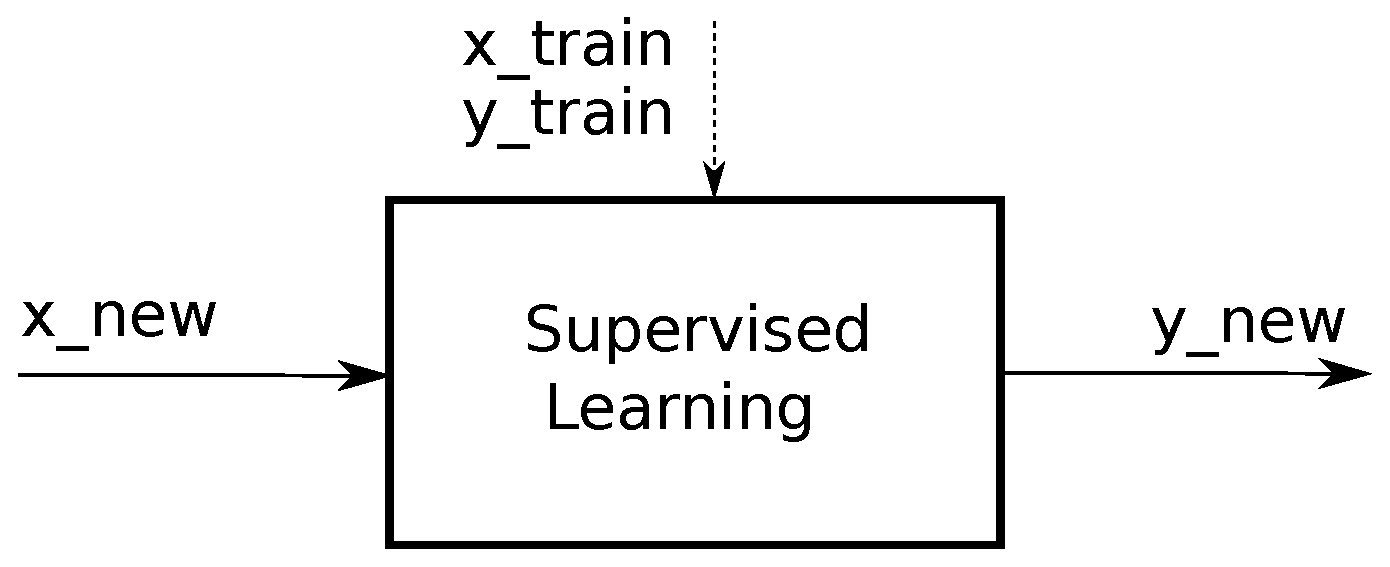
\includegraphics[scale=0.4]{figures/supervisedLearningBlock.eps}
		\caption{Supervised Learning Block Diagram.}
		\end{subfigure}
		\end{center}
		\begin{center}
		\begin{subfigure}{\linewidth}		
		\centering
		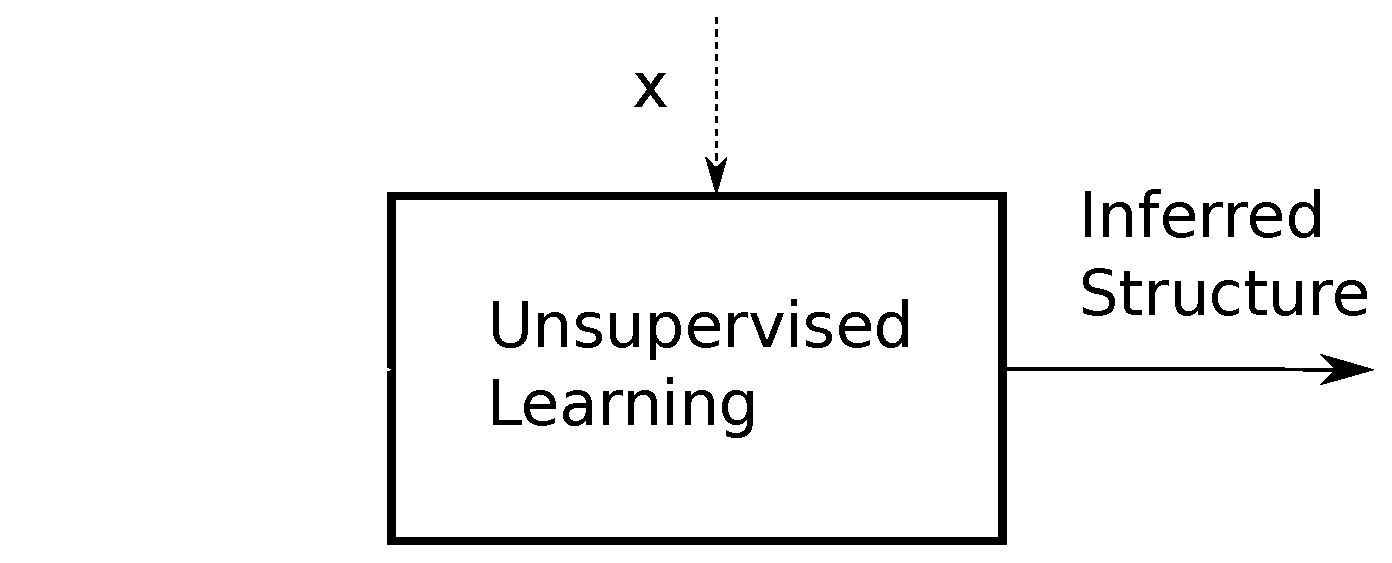
\includegraphics[scale=0.4]{figures/unsupervisedLearningBlock.eps}
		\caption{Unsupervised Learning Block Diagram.}
		\end{subfigure}
		\end{center}
		\begin{center}
		\begin{subfigure}{\linewidth}
			\centering
			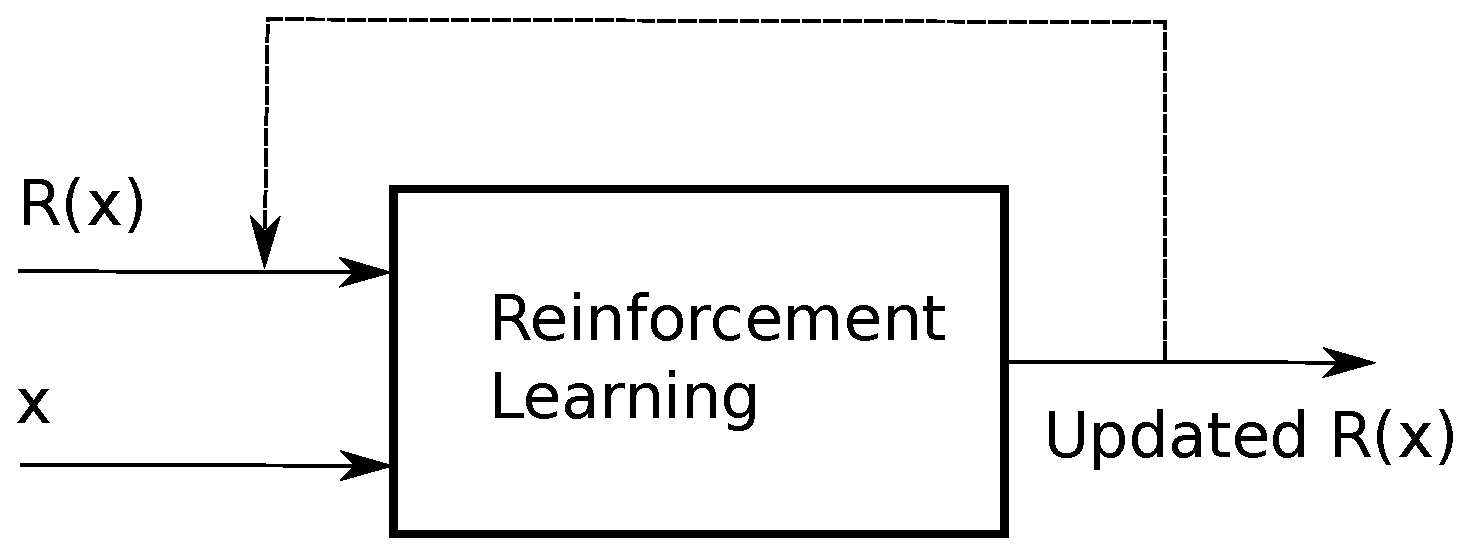
\includegraphics[scale=0.4]{figures/reinforcementLearningBlock.eps}
			\caption{Reinforcement Learning Block Diagram.}
		\end{subfigure}
		\end{center}
		\caption{Flow diagrams of the three main categories of Machine Learning.}\label{bg:SupLearnEx}
	\end{figure}

	\begin{figure}[ht]
		\centering
		\caption{Basic overview of different machine learning techniques.}
		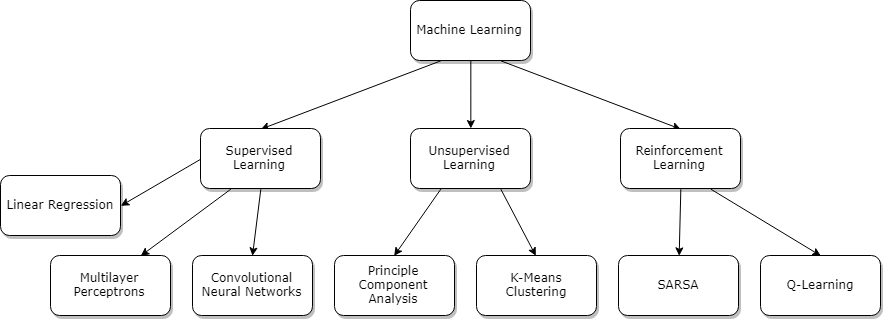
\includegraphics[scale=0.5]{figures/MLdiagram.png}
	\end{figure}
	%\par \textbf{\textit{Decide if I want to include actions as part of RL diagram}}
	
	\par Within the CE, concepts from Supervised Learning and Reinforcement Learning are used. As such, the rest of this section will focus on those two categories in more detail \cite{placeholderCitation}. 
	\subsection{Supervised Learning}
	\par As stated before, supervised learning refers to the problem of modeling some sort of relation between two sets of data: an input dataset and a target dataset. This problem is further subdivided into two different types of problems: regression and classification. Regression refers to the modeling of a continuous target. One common example is the modeling of the cost of a house based on its square footage. $x$ in this case would be the square footage of the house, and $y$ would be the cost of the house. Regression refers to the fact that the cost of a house can have any value within a range. The other type of problem is classification, which models a discrete target. This is the act of assigning input values to one of a number of different classes. A simple to understand example is determining if someone is likely to renew a magazine based on their age. In this case $x$ is the age of the subscriber, and $y$ is whether or not the subscriber will renew their subscription. This is classification because there are two discrete possibilities for $y$, that the subscriber will renew their subscription and that the subscriber will not renew their subscription.  
	\par In order to train a model for either problem class, a set of training data similar to the expected input is required, $X_{train}$. In addition to the input set, the corresponding target values are needed as well, $Y_{train}$. With this information, the chosen algorithm is trained to understand the nonlinear mapping from input to target. Once the algorithm is trained, it will take inputs $X$ and predict the resulting value of $Y$. There are a wide variety of algorithms that are applied to supervised learning. Some relevant algorithms include Linear Regression, Classification and Regression Trees (CART), Multilayer Perceptrons/Feed Forward Neural Networks (MLP/FFNN), and Convolutional Neural Networks (CNN). Each of these algorithms has its own training method. A focused description of the training algorithms for CART and MLP will be provided. CART was chosen because of the relative ease of explanation and the fact that it is often used as a baseline of performance to compare to. MLP was chosen because it is the method used in CE.
	\par The CART is one of the most basic supervised learning techniques still in use today. For each input vector $\vec{x} \in X$, a series of decisions are made based on the values of $\vec{x}$. At each decision, the possible state of the tree is split in two, depending on which value $\vec{x}$ takes. Once there are no more splits, the tree comes to either a class (for classification) or a value (for regression) for $\vec{x}$. This is more thoroughly described in Algorithm \ref{code:bg_cart}.
	\begin{algorithm}[ht]
		\caption{CART Pseudoalgorithm [Note, these variables are not in the text] }
		\label{code:bg_cart}
		\begin{algorithmic}[1]
			\Procedure{CART}{}
			\While{$leafNotReached$}
			\State $x = x_{eval} \in X$
			\If {$x > \textit{branchValue}$} Branch right.
			\Else \ Branch left.
			\EndIf
			\EndWhile
			\State \Return $leafValue$ or $leafClass$
			\EndProcedure
		\end{algorithmic}
	\end{algorithm}

	\par One benefit of this algorithm is that it is fairly intuitive, behaving in a way that is similar to how a human might make a decision. It is also fairly simple, not making any underlying assumptions about the underlying data or requiring any parameters. This allows CART to be applied in a fairly straighforward manner to a wide variety of problems. One downside of CART is that it's simplicity makes the method prone to overfitting. Given $n$ inputs, a tree that splits $n-1$ ways would be capable of 100\% accuracy on the training dataset. However, it would likely underperform on any other data, with stochastic processes or non-generalizable patterns perturbing the data beyond the behavior the tree learned. As a result of this, algorithms must be careful to train only until the tree meets the expected specifications in regards to accuracy and other performance metrics. In addition, pruning techniques to remove non-generalizable branches are employed. When this issue is taken into account, CARTs act as a good baseline algorithm. This has resulted in them being used in many ensemble-based methods, which use multiple copies of an algorithm to produce results. Ensemble-based methods will be discussed in further detail in Section \ref{bg:advanced_ensemble}.
	
	\par While CART is a simple and useful method, the recent resurgence of Machine Learning as a useful field has been driven by extensions of the multilayer perceptron (MLP)\cite{deepLearningSurvey}, also known as the feedforward neural network (FFNN). An MLP is composed of layers. Each layer is itself composed of nodes, each of which holds a value. The inherent meaning of a node value depends on what type of layer the node belongs to. There are three different types of layers: input layers, hidden layers, and output layers. For each MLP there is one input layer, which is composed of inputs $x_i$. Each hidden layer node is a linear combination of all the nodes from the layer before it. How much each node from the previous layer impacts the current node is defined by a set of weights and biases. After this linear combination, the node applies a nonlinear transform, often called the activation function. Frequently, this transform is used as a squashing function to limit the outputs to a certain range\cite{sigmoidReason}. Some examples of this are the tanh() function, which limits the range to (-1,1), and the logistic function, which limits the range to (0,1). Non-linearities are introduced to allow the MLP to represent more complex relationships. Without the activation function, adding additional layers would not result in any increase in representational ability. The output layer takes the values from the last hidden layer and, after one more linear combination, outputs the MLP's prediction of the target value. 
	 % Maybe put a subheader here because it is sort of a break.
	\par In order to train an effective model, there needs to be a way to evaluate how effective the model is at any given moment. For an MLP, this is accomplished by using a cost function $J$, which is used to evaluate how well the model is performing compared to the ground truth. In the context of a classification problem, a commonly used cost function is cross-entropy, also known as log loss. Cross-entropy, a concept taken from information theory, represents the average number of bits needed to identify if a sample was taken from probability distribution $p$ or probability distribution $q$. By choosing $p=y_{truth}$ and $q=y_{pred}$, cross-entropy can be used as a distance metric. A commonly used cross-entropy based cost function is described in Equation (\ref{eq:bg_crossentropy}) \cite{lossFcns}, where $y$ is a binary indicator, with 0 and 1 representing the two different classes that the model is choosing between. By using this formulation, the only factor to loss is the class predicted. 
	\begin{align}
		J_{crossEntropy} &= \frac{\sum_N (y_{truth}log(y_{pred}) + (1-y_{truth})log(1-y_{pred})) }{N} \label{eq:bg_crossentropy} 
	\end{align}
	\par This error function is based on a binary classification problem, but can be easily extended to a multi-class problem by using a separate binary classification for each class, and sum the cross-entropic error for each class to get the total cross-entropic error.  
	\par In the context of a regression problem, a commonly used cost function is mean squared error (MSE). The definition of MSE is given in Equation (\ref{eq:bg_mse}) \cite{lossFcns}. As the name implies, it represents the mean of the squared error between the $y_{pred}$ and $y_{truth}$. Unlike Equation (\ref{eq:bg_crossentropy}), $y$ here represents a continuous value, so the distance of the prediction to the truth value impacts the metric. 
	\begin{align}
		J_{MSE} &= \frac{\sum_N (y_{pred}-y_{truth})^2}{N} \label{eq:bg_mse}
	\end{align}
	\par By using these cost functions, a clearer picture about the effectiveness of a model is created. With training reframed as an optimization problem, the simplest solution is to use gradient descent. Upon taking the gradient of the cost function, the resulting value willbe negative for downward slopes and positive for upward slopes. By updating the weights in the opposite direction of the gradient, the resulting loss value from the updated network will move towards a minimum. This is represented in Equation (\ref{eq:bg_gradDescent}) \cite{backpropIntro}, where $h$ represents the value to change the weights $W$, and $J$ is the Jacobian (the matrix of all first-order partial derivatives of a vector) of the objective function. This method converges well with simpler objective functions, but has the potential to converge slowly, depending on the $\alpha$ parameter and the Jacobian.
	\begin{align}
		h_{gd} &= \alpha J^T W(y_{truth}-y_{pred}) \label{eq:bg_gradDescent}
	\end{align}
	\par Another solution is called the Gauss-Newton method \cite{gauss_newton_alg}, which is applicable to a sum-of-squares objective function, like $J_{MSE}$. It assumes that the objective function is approximately quadratic near the solution, then uses a first-order Taylor series expansion to approximate the Hessian of the objective function to be $J^TWJ$. This then allows for the weight update procedure to follow Equation (\ref{eq:bg_gaussNewton}). This converges much faster than gradient descent for moderately-sized problems, but is only applicable to a stricter set of objective functions, as it depends on the function being twice differentiable. It also doesn't provide as much of a speedup when the first derivative of the objective function has repeated roots. 
	\begin{align}
		h_{gn} &= (J^TW(y_{truth}-y_{pred}))(J^T WJ)^{-1} \label{eq:bg_gaussNewton}
	\end{align}
	\par The solution that is frequently used (and is the MATLAB default in training a neural network) is the Levenberg-Marquardt method\cite{lm_alg}. This is effectively a combination of the two prior optimization methods. It is described in Equation \ref{eq:bg_lm}. 
	\begin{align}
		h_{lm} &= (J^TW(y_{truth}-y_{pred}))(J^T WJ + \lambda \cdot diag(J^T WJ))^{-1} \label{eq:bg_lm}
	\end{align}
	\par The variable $\lambda$ represents the parameter that controls how similar the update is to Gradient Descent, and how similar the update is to Gauss-Newton. A large $\lambda$ makes LM more similar to Gradient Descent, and a small $\lambda$ makes LM more similar to Gauss-Newton. The variable $\lambda$ is usually initialized to be large, to enable the first updates to be small. If an update increases the objective function, than $\lambda$ is increased, moving closer to Gradient Descent. Otherwise, $\lambda$ decreases, moving closer to Gauss-Newton. This is reasonable because as the weights approach the optimal solution, it is more reasonable to assume that the cost function is quadratic.
	\par For an algorithm like linear regression, one of these update methods by itself is enough as an update procedure. However, MLPs require a modification of this process. This is due to the multiple layers involved, which introduce additional complexity with the interconnections between layers. The process of updating FFNNs is called Backpropagation. Gradient Descent Backpropagation will be described in Algorithm \ref{alg:bg_gdBackprop}, as it is the simplest to understand. Backpropagation as applied to Levenberg-Marquardt can be found in \cite{placeholderCitation}.
	%label{code:bg_backprop}
	\begin{algorithm}
		\caption{Pseudocode for Backpropagation}
		\label{alg:bg_gdBackprop}
		\begin{algorithmic}[1]
			\State Given: training set $X$.
			\Procedure{Backpropagation}{}
			\State Set input activation $a^1=\sigma(X)$
			\For{$l=2$:$L$}
			\State $z^l = w^l a^{l-1} +b^l$
			\State $a^l = \sigma(z^l)$ 
			\EndFor
			\State $\delta^L = \nabla_a C \odot \sigma '(z^L)$
			\For{$l=L-1$:$2$}
			\State $\delta^l = (w^{l+1}\delta^{l+1}) \odot \sigma '(z^l)$
			\EndFor
			\State Output 1: $\frac{\delta C}{\delta w^{l}_{jk}} = a^{l-1}_{k}\delta^{l}_{j}$
			\State Output 2: $\frac{\delta C}{\delta b^{l}_{j}} = \delta^{l}_{j}$
			\EndProcedure
		\end{algorithmic}
	\end{algorithm}
	\par The symbol $\odot$ is the Hadamard Product, which is an element-wise product of two vectors with the same length. $L$ is the number of layers in the MLP. $z^l$ is the weight and bias values at layer $l$, and $a^l$ is $z^l$ passed through the activation function $\sigma(z)$. $\delta^l$ is the error at layer $l$.
	\par The backpropegation algorithm used in MLPs can be broken into 4 steps: forward propegation, backpropegation at the last layer, backpropegation at the hiden layers, and updating of the weights. 
	Forward propegation is simply applying the training inputs to the network as normal (represented by steps 2-6). Then, the backpropegation error at the output is calculated (step 7). Then, the error is carried back through the network in the same way that the MLP is applied, except backwards. Once this is done, the partial derivatives of each node will be calculated, and can be used in a gradient descent manner. 
	\begin{figure}
		\centering
		\caption{A flow diagram describing gradient descent.\textit{\textbf{[make a flow diagram ]}}}\label{bg:flowBackProp}
		
\includegraphics[scale=0.5]{figures/Placeholder.png}
	\end{figure}
	\par In recent times, improved versions of backpropegation have been proposed and utilized, such as RMSprop and Adam. Both of these improvements are extensions of standard gradient descent backpropegation. Standard backpropegation utilizes one learning rate for all weight updates. This rate doesn't change during training. RMSprop, also known as Root Mean Square Propagation, maintains per-parameter learning rates that get adjusted by a moving average of the recent gradient values for the individual weight \cite{RMSPropPaper}. Adam takes this a step further and adapts the parameter learning rates based on the gradient's variance, in addition to the gradient's mean that RMSProp uses. Doing so results in quicker convergence than standard backpropegation. Details can be found in \cite{AdamPaper}. In modern times, Adam has been frequently recommended as the default optimization method in training neural networks\cite{CNNKarpathyClass}. Both RMSProp and Adam are still based on first-order methods, unlike Gauss-Newton and Levenberg Marquardt, which is likely one of the reasons why the new algorithms have surpassed the old ones in usage. Nonetheless, the same concern in online usage remains. This thesis will stick to LM, as the project it is building on top of is based off of LM.
	\par http://cs231n.github.io/ karpathy CNN class
	\par https://page.mi.fu-berlin.de/rojas/neural/chapter/K7.pdf Link to chapter that discusses backprop
	\subsection{Reinforcement Learning}

	\begin{figure}
		\centering
		\caption{An overview of reinforcement learning.\textit{\textbf{[Get figure from paulo's RL diagram]}}}\label{bg:flowRL}
		
\includegraphics[scale=0.5]{figures/Placeholder.png}
	\end{figure}

	\par While both supervised and unsupervised learning are built on the premise of identifying some form of structure from a given set of data, the goal of Reinforcement Learning (RL) is fundamentally different. The core premise of RL is of an agent trying to learn an environment. In passive RL, there agent has no influence on the environment, and can just observe some reward based on the location it is at. In active RL the agent is able to take actions, and so the reward is based on the location and the action that was taken. With this reward value, the agent can update its understanding of the environment, in a form called the state-transition model. How it does this depends on the RL algorithm being used. Active RL is more relevant to this thesis
	\par While there are multiple different ways to pose an RL problem, the one that is most applicable to the problem at hand is the Multi-armed bandit. In this model, an action set has multiple reward functions, used as metrics for how well a task was executed. 
	The agent is the "bandit", trying to get the "best" reward overall over the multiple reward functions. How best is defined is difficult, as the interaction between reward functions is not straightforward, and the impact of each reward function may vary. 
	 Another potential model is that of a state-transition problem, modeled as a Markov decision process. Rephrased in a RL context, the target problem is changing radio parameters so that optimal performance is achieved in context of the current environmental conditions. There are a wide range of conditions that affect the state-transition model, including the communications channel. This channel is affected by the dynamic geometry of the line-of-sight between the transmitter and receiver, as well as atmospheric and space weather. These complex and changing conditions make finding the state-transition model and action-state mapping analytically an intractable pursuit. 
	\par This difficulty is what makes RL a good fit for tackling the problem. RL makes few assumptions about the behavior of the process being studied, other than the fact that it can be reasonably modelled by a state-transition model. In addition, RL is designed to be constantly used and updated, instead of waiting for the optimal solution to be calculated before running. With these two properties, the primary concern shifts from intractability to ensuring the agent interacts with the environment in an efficient way to find the best possible policy. The best way to form a policy would be to evaluate the action-value function $Q(s,a)$ at each possible state and action. However, this becomes intractable quickly. Instead, the agent periodically explores policies, with either on-policy or off-policy approaches. On-policy approaches affect the policy that the agent uses to make decisions, while off-policy approaches affect a separate policy from the one that the agent uses to make decisions. Since the target platform is a cognitive engine that actively adapts to the environment conditions, the focus will be on-policy approaches. 
	\par The model-free method that is relevant to this thesis is Temporal-Difference (TD). This method updates $Q(s,a)$ using the past experiences at each time step. This makes it useful for time-sensitive applications. When used on-policy, it is called State-Action-Reward-State-Action (SARSA). The pseudoalgorithm for SARSA is provided in Algorithm \ref{code:bg_SARSA}.
	
	\begin{algorithm}[ht]
	\caption{SARSA Pseudoalgorithm}
	\label{code:bg_SARSA}
	\begin{algorithmic}[1]
		\Procedure{SARSA}{}
		\State Initialize $Q(s,a)$ for all states $s$ and actions $a \epsilon \mathcal{A}(s)$ arbitrarily. Set $Q(terminal\ state)=0$.
		\While{Learning}
		\State Initialize $s$
		\State Choose $a$ from $s$ using policy derived by $Q$.
		
		\While{not terminal state}
		\State Take action $a$, observe reward $r$ and next state $s'$.
		\State Choose $a'$ from $s'$ using policy derived from $Q$.
		\State Update Q: $Q(s,a) \gets Q(s,a) + \alpha[r + \gamma Q(s',a')-Q(s,a)]$.
		\State Update $s \gets s'$,$a \gets a'$.
		\EndWhile
		\EndWhile
		\State \Return Updated Q table.
		\EndProcedure
	\end{algorithmic}
\end{algorithm}

		\par $\alpha$ is the learning rate of the algorithm, r is the reward, $\gamma$ is the discount factor for future rewards. In our context, there is no terminal state. The algorithm instead ends when there is no longer a connection between the SCaN testbed and the ground station. Described briefly in words, the SARSA algorithm is as follows. Before running, initialize the Q function for all possible states and actions. Then, initialize the current state, and choose a based on a given policy. Take the action $a$, and observe reward $r$ and state $s'$. Using the same policy based on Q, choose the next action $a'$ given $s'$. From this, update $Q(s,a)$. The value within the brackets is known as TD error, and is the difference between the predicted value of $Q(s_k,a_k)$ and the better prediction of $r + Q(s_{k+1},a_{k+1})$. Then, repeat the process of taking actions and observing rewards. 
	\par In the context of cognitive radio, only the immediate reward ($\gamma = 0$) is relevant \cite{AIAA_Paper}. In addition, any action can be taken from any state, without the need for planning. This results in a modified Q function, Equation \ref{eq:bg_sarsa2}.
	\begin{align}
		Q_{k+1}(s_k,a_k) &= Q_k(s_k,a_k) + \alpha[r - Q(s_k,a_k)] \label{eq:bg_sarsa2}
	\end{align}
	\par Beyond $Q(s,a)$, a reward function $r = g(s,a)$ and an exploration policy $a = h(s)$ need to be defined before a practical model is complete. In the context of the CE, a multitude of performance functions are relevant to the overall performance of the system. These performance functions may or may not have conflicting responses. The reward function mapping environmental information to performance is a combination of values from these performance functions. The overall result is then represented as a percentage of the maximum possible performance value.   
	\par In a standard RL system, a knowledge base, or Q-table, is built up. In this Q-table, previous Q-values are mapped to state-action pairs. This table is what gets updated by SARSA. \textbf{\textit{[check if this needs more context]}}
	
	\par In RL, one of the most important tradeoffs is deciding how much time should be spent exploring the environment versus how much time should be spent exploiting the knowledge already gathered. This is frequently called the Explore-Exploit tradeoff. In the context of SARSA, exploring would represent choosing an unvisited action, while exploiting would be choosing an action that has the highest Q value. The exploration policy is responsible for making this decision. This tradeoff is important because exploring too much would create a detailed understanding of the environment, but would not actually use the information, while exploiting too much could be using subpar information, as the environment is only explored a little bit. The preventing of either of these cases becomes an important issue. 
	\par There are many different approaches to tackling the explore-exploit tradeoff. The simplest one is to use an $\epsilon$-greedy policy. In this method, an $\epsilon \in (0,1)$ is chosen, which is the probability of choosing a random action. Otherwise, a greedy action based on the Q-table is chosen. $\epsilon$ can be set as a function of time, resulting in more exploration at the beginning of an algorithm, and more exploitation as time goes on and more of the environment is explored. Other plicies include value-difference based exploration (VBDE), which changes $\epsilon$ based on TD error, as well as Boltzmann exploration, probability matching, etc. In this work, a time-varying $\epsilon$-greedy policy is used. 
	
	\section{Previous work on NASA SCaN Testbed}
	\par This section first describes the problem that is trying to be solved by the NASA John H. Glenn Research Center (GRC) Space Communications and Navigation (SCaN) Testbed project. With this foundation, the architecture of the cognitive engine (CE) that was developed will be described as well. Finally, the primary goals of the extension that this thesis is focused on will be described.
	\subsection{Problem statement}
	\par The Cognitive Engine project, and by extension this thesis, is built on top of the SCaN Testbed, an experimental communication system developed by NASA to research implementation solutions for issues related to SDR-based communications to and from space. The platform consists of multiple SDRs that are configured to operate at S-band and Ka-band, both in direct communications to ground stations on Earth and in communication with NASA's satellite relay infrastructure named Tracking and Data Relay Satellite System (TDRSS). For this thesis, communication with ground stations is the central focus. This platform is used to research real-world satellite dynamics between spacecraft and relay satellites or ground stations. Some of the dynamics studied include time-varying Doppler changes, differences in thermal conditions, interference, range variation, ionospheric effects, and other impairments to propagation.
	\par The SDRs chosen for the SCaN testbed are flight-grade systems, fully compliant with NASA's Space Telecommunications Radio System (STRS) SDR architecture. This architecture provides abstraction interfaces between the radio software and proprietary hardware, allowing for third-party software waveforms and applications to interact with and run on the radio. In the context of communications systems, waveforms refer to the specific PHY standards used when transmitting a message, including the configurable parameters that they specify are allowed. \textbf{\textit{[Is this an accurate description of waveforms? I'm mainly getting it from intuition based on how other people talk about waveforms. -Max ]}} STRS also provides a library of waveforms available that provide various modulation, coding, framing and data rate options. 
	\par On top of this platform, solutions such as adaptive communications using cognitive decision making can be researched. Doing so will help solve communication issues on Earth, as well as allow for the development of space communication systems that will enable space exploration in the near future \cite{paulo_cite_131}. SDRs are important in this development, as their flexibility and reconfigurability provides a strong tool that enables a wide variety of tests. However, SDRs tend to be more complex than traditional fixed-configuration radios. Cognitive radio (CR) systems help reduce the complexity and risk in using these systems. The work that this thesis is extending plays a part in this effort, providing CR algorithm research for SDR systems in space.    
	\par Three areas have emerged as candidate application areas for the application of CR: node-to-node communications, system-wide intelligence, and intelligent internetworking. The first application focuses on radio-to-radio links between mission spacecraft and a ground terminal. Cognitive decisions may improve throughput across the communication link by adjusting waveform settings to maximize user data and symbol rate, while using more conservative settings during parts of the pass with poor channel conditions. The second application is system-wide intelligence, where the CR systems make operational decisions normally performed by operators. For instance, CR systems could be applied to scheduling, asset utilization, optimum link configuration and access times, fault monitoring, and failure prediction, among others. In this application, a CR system could reduce operation oversight and reduce operational complexity, by choosing among the large search space of configurations. The final application of CR systems applies to the network level. With control and data functions of the communications network, CR systems could optimize data throughput using QoS metrics such as bit error rate. Learning network behaviors could enable the CR to provide throughput and reliability benefits.
	\par  For this thesis and the work preceding it, the first application is the main priority. However, regardless of the application, the need for verification and ground-testing of all operational conditions before launch becomes apparent. Doing so minimizes the risk of malfunction on-orbit. Once this verification is complete, tests (including the one in this thesis) can be conducted in order to more properly study the impact of CR systems on communications.
	\par The project that this thesis is extending, titled "Intelligent MAC protocol for SDR-based satellite communications", was accepted by NASA Glenn Research Center (GRC) in order to develop a cognitive engine algorithm for future space-based communications systems. With this acceptance came the opportunity to perform on-orbit tests with the SCaN Testbed SDRs. The R\&D team is composed of members from WPI and the Pennsylvania State University, in collaboration with the SCaN team at NASA GRC. The project commenced in November 2014, and the initial tests were completed in May of 2017. This extension is scheduled to be completed by December of 2018.
	\par During the course of this project, the team has designed and developed a proof-of-concept of an intelligent MAC protocol to maximize data link performance and improve robustness of space communications systems. This uses SDRs for low margin data links operating on dynamically changing channels. The protocol's core is made of a Cognitive Engine (CE) that balances multiple different objective issues during radio-resource allocation. Radio parameters may be adapted to mitigate channel impairments or when meeting new performance requests.Key capabilities for cognition are prediction and learning techniques, assisted by third-party databases when they are available.  
	\par This CE project is aligned specifically with NASA's Communication and Navigation Systems Roadmap Technology Area 5 \cite{placeholderCitation}, which focuses on cognitive radios in space that sense the environment, autonomously determine when there is a problem, attempt to fix it, and learn about the environment as they operate. It also acts asa step towards reducing the limits that communication techniques impose on future missions and their critical phases. The CE algorithm, as well as expreiment results, will be used to asses the performance of the adaptive MAC protocol performance for on-orbit SDRs, and will help in the design of future MAC protocols and mitigation techniques that utilize intelligent radio parameter reconfiguration. 
	\par There are four different communication channels between the fixed ground stations at GRC/White Sands, the moving ScaN Testbed SDR on board the ISS, and the TDRSS satellite at a GEO orbit, as illustrated by Figure \ref{fig:exampleCommChannels}. Radio parameter reconfiguration might be done during periods of signal fading, especially those happening during low elevation angles of the SCaN Testbed antenna, while tracking the TDRS satellite, or low elevation angles from a GRC ground station antenna, while tracking the ScaN Testbed. The project focuses on the direct communication between GRC and the SCaN Testbed.
	\begin{figure}
		\centering
		\caption{Four potential communication channels.}\label{fig:exampleCommChannels}
		
\includegraphics[scale=0.5]{figures/Placeholder.png}
	\end{figure}
	\begin{figure}
		\centering
		\caption{A flow diagram describing the CE's flight-test setup.}
		\label{fig:CE_outline}
		
\includegraphics[scale=0.5]{figures/system_block_diagram.eps}
	\end{figure}
	
	\par A high level overview of the proposed CE is shown in Figure \ref{fig:CE_outline}. The platform gathers telemetry data reported from the transmitter or measured at the receiver. A predictor uses past information to predict which radio parameter values will achieve good performance. Learning techniques are used for prediction in order to control storage memory growth. Decision logic based on the predictions will choose what adaptations will need to occur. The CE learns the environment behavior by building a model that maps observed telemetry data to radio parameter sets. The CE is shown in more detail in Figure \ref{make this figure too}, it will be discussed in more detail in Section \ref{reference to the methods chapter}.
	\begin{figure}
		\centering
		\caption{An overview of the CE.\textit{\textbf{[make MAKETHISFIGURE, eg the CE diagram figure]}}}
		\label{bg:CEFigure}
		
\includegraphics[scale=0.5]{figures/Placeholder.png}
	\end{figure}

	\par In this thesis, the goals were twofold: to explicitly deal with the catastrophic forgetting that occurs in MLPs, and to investigate the potential utility of GANs. In the following section, both of these subjects will be discussed in more detail.
	
	\section{Advanced Topics in Machine Learning}
	\subsection{Online Learning and Catastrophic Forgetting}
	\par In supervised learning, there are two different learning paradigms: online learning and offline learning. Offline algorithms assume that there is one set of inputs and outputs to train on, and that once training is complete that there will be no updates to the algorithm. The training methods described in Section \ref{bg:introToML} are all considered offline methods. This is contrasted with online algorithms, that update as new data is received. The choice between an offline algorithm and an online algorithm is dependent on the problem that is selected. With a stationary dataset, a single training period can be sufficient. However, if the dataset is nonstationary, there is reason for multiple training periods that capture the shifting of the data, also known as concept drift. Because effective space communications systems are dependent on many nonstationary variables, online methods are more suited for this project.
	\par The most basic category of online methods consists of generalizations of offline methods. In this category, a window of incoming data is collected. Once this window is full, the collected data is used to train using an offline method. Then, some number of datapoints are dropped, and the window is filled again. This moving window process is the most straightforward extrapolation of offline algorithms. In the baseline CE, this method is applied to Levenberg-Marquardt. The moving-window approach has one major problem that it introduces. The LM algorithm updates the weights completely using the data that is put into it. Many first-order offline algorithms work in a similar manner (SGD, ADAM, RMSProp, etc.). In this type of online method, the window moves and overwrites old datapoints, with these old datapoints no longer influencing how the model is trained. Because of this, the model will lose the information that was encoded as a result of these datapoints. This is called catastrophic forgetting.  Catastrophic forgetting primarily affects learning in non-stationary environments. If an environment is stationary, the fact that datapoints are no longer used in training has little effect, as the datapoints replacing them will come from the same probability distribution. In non-stationary environments, however, the loss of information is more significant. If there is any cyclical nature of the changes, the information will have to be relearned each time.
	\begin{figure}[ht]
	\centering
	\begin{subfigure}{\linewidth}%[First training. Since no training has occurred beforehand, the entire training buffer is used.]
			\centering
			
\includegraphics[width=\textwidth]{figures/CatastrophicForgettingA}
			\caption{First training. Since no training has occurred beforehand, the entire training buffer is used.}
	\end{subfigure}
	\begin{subfigure}{\linewidth}
		\centering
		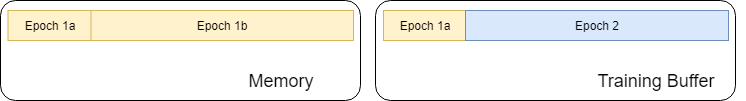
\includegraphics[width=\textwidth]{figures/CatastrophicForgettingB}
		\caption{Second training. Some of the first training epoch is kept, but most of it is replaced by new data from epoch 2.}
	\end{subfigure}
	\begin{subfigure}{\linewidth}
	\centering
	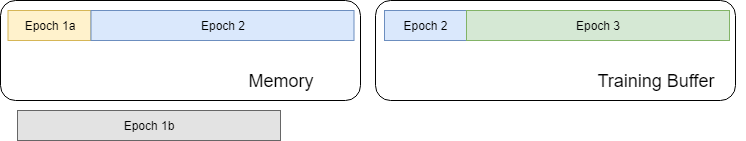
\includegraphics[width=\textwidth]{figures/CatastrophicForgettingC}
	\caption{Third training. All data from epoch 1 is no longer kept, and only data from epoch 2 is in the training buffer. A portion of epoch 1 is no longer in the memory of the MLP.}
	\end{subfigure}%
	\caption{A visual representation of how catastrophic forgetting occurs.}
	
	\end{figure}
	\par One way to deal with this is to use a recursive training method. This updates the network based on batches of samples each time, but uses these samples to update an internal state. The recursive implementation LM, as described by Ngia and Sjoberg \cite{placeholderCitation}, is used in this thesis. In this process, there is a forgetting factor $\alpha$ built in, allowing for the network to forget past inputs in a more explicit manner than the standard batch-update method. In the following equations, $\varepsilon(h_t) = \sqrt{J(h_t)}$, $P_t$ can be considered the covariance matrix of the weights, $\Omega^T(h_t)$ is a modified gradient for y, allowing for a normalization factor $\rho$ to be added in one weight at a time. The second row of $\Omega^T(h_t)$ is 0 for all indices where $i\ mod\ (nWeights+1) \neq t$, and 1 where $i\ mod\ (nWeights+1) = t$. $\alpha$ is the rate of forgetting. 
	\begin{align}
		\Omega^T(h_t) &= \begin{bmatrix}
			&& \nabla_y^T(h_t) && \\ 0 & ... & 1 & ... & 0
		\end{bmatrix} \\
		\Lambda_{T}^{-1} &= \begin{bmatrix}
			1&0\\0&\rho
		\end{bmatrix} \\
		S(h_t) &= \alpha_t\Lambda_t + \Omega^T(w_t)P_{t-1}\Omega(w_t) \\
		P_t &= \frac{1}{\alpha_t}[P_{t-1}-P_{t-1}\Omega(h_t)S^{-1}(h_t)\Omega^T(h_t)P_{t-1}]\\
		h_{t+1} &= h_t + P_t \nabla_y(h_t)\varepsilon(h_t) 
	\end{align}
		\textbf{\textit{REVISIT, include pre-recursive formulation.}}
	\par The update process is split into three substeps, each substep updating a a related aspect of the internal or external state of the NN. The first step computes an intermediate state $S(h_t)$, which reduces the necessary matrix inversion to a 2x2 matrix. The second step updates the covariance matrix, and finally the third step updates the weights. 
	\subsubsection{Ensemble Learning}\label{bg:advanced_ensemble}
	\textbf{\textit{Don't forget to cite cart in this bg section \cite{cartIntro}}}
	\par A different approach to deal with Catastrophic Forgetting is to use ensemble training methods. Ensemble methods use a collection of learners to produce improved results over any individual learner by itself. In general, ensemble methods use a set of weaker algorithms that are combined with or without some sort of weighting to produce a unified result. In classification problems a weighted majority voting is often used, while in regression problems a weighted median or mean is often used. Frequently, a CART is used as the base algorithm, due to its simple implementation and reasonable performance. However, any algorithm can be selected. Once a base algorithm is chosen, the difference between ensemble implementations is how the ensemble is created and used. For instance, in Adaboost, a series of base learners is trained, with each successive base learner trained in a way that more heavily weights points that the previously trained learners have trouble with. This differs from bagging, a different algorithm where each base learner is trained with a different subset of the total training data. These examples are provided simply to show how ensemble learning methods can differ.
	\par The method most relevant to addressing the problem of catastrophic forgetting is Learn++.NSE. For each window of samples, Learn++.NSE creates a new learner, trained on the window. The samples in the training window are weighted by how much trouble the pre-existing learners had in predicting the value, ensuring that the new learner is better at recognizing these samples. It then weights the new learner and existing learners based on how well they work on the training data, using a metric such as MSE. In doing this, existing learners contribute to the resulting prediction based on how well they work on the most recent window of data. 
		\begin{algorithm}[ht]
		\caption{Learn.NSE++ Pseudoalgorithm}
		\label{code:bg_nse}
		\begin{algorithmic}[1]
			\Procedure{Learn.NSE++}{}
			\State $t=1,\ numActiveClassifiers = 0$ 
			\State $m^t$ is the data window size at epoch t.
			\While{Running}
			\If{$t = 1$} 
			\For{$i=1 \to numActiveClassifiers$}
			\State $D(i) = w(i) = 1/m^1$
			\EndFor
			\Else
			\State Apply data window to current ensemble. 
			\State $E^t = \sum^{m^t}(1/m^t) * squaredError($current learner, current data$)$
			\State At this point, $E^t$ should be a vector with size $m^t$.
			\For{$i = 1,i<numActiveClassifiers, i++$}
			\State Update learner weights: $w_i = 1/m^t * \sum squaredError($current learner, current data$)$
			\EndFor
			\State Normalize learner weights: $D = w \odot (1/\sum w)$
			\EndIf
			\If{ $numActiveClassifiers = numClassifiers$}
			\State Remove oldest classifier.
			\Else
			 $numActiveClassifiers = numActiveClassifiers + 1$
			\EndIf
			\State Train new Learner on new data window.
			\State Evaluate all existing classifiers with new data.
			\For{$i=1 \to numClassifiers$}
			\State $\epsilon_i^t = \sum D(i) * squaredError($ current learner, current data$)$
			\State $\beta_i^t = \epsilon_i^t/(1-\epsilon_k^t) $
			\State Compute average of normalized error for $h_i$: $\omega_i^t = 1/(1+exp(-a(t-i-b)))$
			\State $\omega_i^t = \omega_i^t / \sum_{j=0}^{t-i} \omega_i^{t-j}$
			\State $\hat{\beta_i^t} = \sum_{j=0}^{t-i} \omega_k^{t-j} \beta_i^{t-j}$
			\If{$t>numClassifiers$} 
			\State Calculate classifier voting weights $W_i^t = log(1/\hat{\beta_i^t})$
			\EndIf
			\EndFor
			\State Training Done.
			\While{Filling training buffer}
			\State get Hypothesis $H(x) =\sum_{i=0}^{numClassifiers} W_i^t * h_i(x) $
			\EndWhile
			\State Buffer full, $t += 1$.
			\EndWhile
			\EndProcedure
		\end{algorithmic}
	\end{algorithm}
	\par In the standard implementation of Learn++.NSE, a classification problem is targeted, and it is supposed that an infinite number of learners can be created. The adjustment from classification to regression required the algorithm to use MSE instead of cross-entropy as an error function, and a method for limiting the number of learners was required as well. Due to time constraints, a simple pruning process of choosing a maximum number of learners and replacing the oldest learner was chosen. More complex pruning methods can be explored in \cite{placeholderCitation}.
	\subsection {GANS, and evaluating the utility of them}
	\par One of the major goals of this extension to the previous work is to evaluate if the concept of Generative Adversarial Networks, or GANs, was applicable to the project. Like the cognitive engine in its current state, GANs are composed of two neural networks, providing complementary data. In this section, GANS will be described in more detail, as well as their applicability to the CE.  
	\par The primary purpose of a Generative Adversarial Network is to implicitly model some probabilistic data distribution. This is usually done in the case where data is either too complex to model effectively or completely unknown. Prior work has focused primarily on image-based data. Common datasets to be modeled for testing include MNIST (hand written digits), CIFAR-10 (natural images) and the Toronto Face Dataset (TFD) \cite{gan_overview}. These distributions happen to be all image-based, but there is no explicit need for the data distribution to be an image. Images just happen to be an extremely complicated representation space with many nonlinear patterns, making it a good data type for practice.
	\par A GAN is composed of two separate learners, a Generator($\mathcal{G}$) and a Discriminator($\mathcal{D}$). $\mathcal{G}$ and $\mathcal{D}$ are configured to be in competition. $\mathcal{D}$ is attempting to distinguish between points that are generated by $\mathcal{G}$ and points that are sampled from the true distribution. $\mathcal{D}$ returns a 0 if it thinks the datapoint is not from the true distribution, and a 1 if it thinks the datapoint is. $\mathcal{G}$ is attempting to fool $\mathcal{D}$ into confusing its generated datapoints with the data from the true distribution. Its best case scenario is that $\mathcal{D}$ is only correct around 50\% of the time, as this makes $\mathcal{D}$'s prediction as good as randomly guessing which distribution the sample is from.
	\par In a more formal sense, $\mathcal{D}$ can be considered as dealing with a standard classification problem, attempting to classify whether or not a sample it is given is from the real distribution or the artificial one. $\mathcal{G}$ can be considered as dealing with a regression problem, trying to map a random uniform input $U(0,1)$ to the true distribution. 
	\par Figure \ref{bg:fig_ganDiagram} shows an overview of the GAN architecture. The task of $\mathcal{G}$, modeling a probability distribution, is more difficult than the task of the discriminator, $\mathcal{D}$, classification of incoming data. As such, when the discriminator ceases to improve, it is often frozen, and only $\mathcal{G}$ gets updated. 
	\par The training of GANs is based on a value function $V(\mathcal{G},\mathcal{D})$ that's dependent on both the generator and the discriminator. Training the GAN accomplishes the following: 
	\[ \max_\mathcal{D}\min_\mathcal{G} V(\mathcal{G},\mathcal{D}) \] where
	\begin{align}
		V(\mathcal{G},\mathcal{D}) &= E\{p_{real}\}log(\mathcal{D}(x)) + E\{p_{generated}\} log(1-\mathcal{D}(x))
	\end{align}
	\par The competing nature of $\mathcal{G}$ and $\mathcal{D}$ is shown by the fact that one is rying to maximize the value function while the other is trying to minimize it. The first part of $V(\mathcal{G},\mathcal{D})$ represents the log-probability that the discriminator successfully classifies real datapoints as real. The second part represents the log-probability that the discriminator successfully classifies generated datapoints. $\mathcal{D}$ is thus trained by ascending the gradient of $V(\mathcal{G},\mathcal{D})$, and $\mathcal{G}$ is trained by descending a modified version of the gradient. Since $\mathcal{G}$ is only able to affect the probability of $\mathcal{D}$ providing a false positive, it only attempts to minimize this part of $V(\mathcal{G},\mathcal{D})$. This becomes:
	\begin{align}
		\min_\mathcal{G} E\{p_{generated}\} log(1-\mathcal{D}(x))
	\end{align}
	\par In order to use a non-saturating criterion, the minimization is rearranged to be a maximization, as shown in Equation (\ref{eq:bg_nonsatG}):
	\begin{align}
		\max_\mathcal{G} E\{p_{generated}\} log(\mathcal{D}(x)) \label{eq:bg_nonsatG} 
	\end{align}
	
	%\textit{\textbf{NOT SURE IF SHOULD REFRAME X TO BE G(z) IN THIS OR NOT}}
	\par Beyond the value function, standard gradient-based backpropagation methods are used for updating the networks. Both networks are trained in tandem: a batch of real samples is collected, a batch of generated samples are created, and then the results of feeding these samples through $\mathcal{D}$ are used to update both $\mathcal{D}$ and $\mathcal{G}$.  
	\begin{figure}
		\centering
		\caption{A flow diagram describing how GANs are structured.}
		\label{fig:GanFlowDiagram}
		
\includegraphics[scale=0.5]{figures/Placeholder.png}
	\end{figure}
	\par While GANs are a versatile method for modeling a data distribution, the training process is far from robust. The first issue is that there is no guarantee that the pair of models will converge. Because of the adversarial nature of the network, the convergence of a GAN  depends on both models converging with competing objectives. The standard GAN procedure does not have any guarantees that this will happen. Another issue is mode collapse, when $\mathcal{G}$ starts to produce very similar samples for different inputs. This may result in good values for $V(\mathcal{G},\mathcal{D})$, but will only model a specific subset of the real data distribution. A final issue is that the loss value of $\mathcal{D}$ can quickly converge to zero, making there no reliable way to update $\mathcal{G}$. This is called the Vanishing Gradient problem, and is not specific to GANs. 
	\par In practice, there are a couple of approaches that are used to reduce the impact of these issues. One method is to normalize the inputs of each layer by subtracting the input mean and dividing by the input standard deviation. This ensures that inputs of vastly different magnitudes can be represented in a more similar manner. Doing this introduces a "standard deviation" parameter and a "mean" parameter for each node, allowing for the training process to use "denormalized" nodes if it's optimal, without reducing the overall stability. This most directly affects the Vanishing Gradient problem, but also has positive effects on convergence rate as well.
	\par An approach used to deal with mode collapse is mini-batch discrimination, which adds an input to the discriminator that encodes the distance between a sample in a mini-batch and the other samples. This makes the discriminator able to tell if the generator is producing the same outputs. Another approach, called feature matching, alters the goal of $\mathcal{G}$ to try to match an intermediate activation of $\mathcal{D}$ from real samples with its generated samples. The additional information makes it more able to represent complex representations. Heuristic averaging, which penalizes network parameters if they stray from a running average of previous values, is a useful approach to aid in making the GAN converge. 
	\par Beyond the heuristic approaches, there have been a few attempts at alternative, more robust formulations of GANs. The most prominent approach is the WGAN \cite{bg:wganPaper}. This modifies the cost function of the GAN to use Wasserstein distance, instead of cross-entropy. The details of Wasserstein distance, also known as Earth-Mover distance, are irrelevant to this thesis, and so will be left for viewer investigation. However, the intuition of Wasserstein distance is that:  
	\begin{itemize}
		\item $P_x$ and $P_y$ are similar to piles of earth. 
		\item $\gamma(x,y)$ is the amount of "mass" that needs to be moved to make $P_x$ into $P_y$.
		\item Wasserstein distance is the "cost" of the optimal transport plan of $\gamma$.
	\end{itemize}
	Other interesting alternate GANs are DCGAN and ALI.
	\par On a surface level, the RLNN has some similarities to the GAN. Like a GAN, the RLNN uses two neural networks working in combination to produce different types of results. However, many of the similarities end here. The performance of the explore and exploit networks are not particularly related, as the performance of one doesn't indicate the performance of the other. Furthermore, neither the explore network nor the exploit network were developed as a classification problem. In order to make these networks fit the GAN structure, there would need to be a restructuring of the RLNN architecture.
	\par Another potential way to use the GAN is in replacement of the explore or exploit network. The Explore network is the model that fits into the standard GAN formation. Indeed, it could be considered to be attempting a similar problem as $\mathcal{G}$. While there would be benefits of replacing the Explore network with a GAN, limitations of the experiment setup prevent doing so. The amount of samples required to properly train a GAN would likely be prohibitive, considering how difficult it is to schedule time to conduct experiments on the space-based platform. As a result of this, the conclusion is that GANs are not directly applicable to the SCaN testbed CE.
	
%\end{document}
	\chapter{Methods}\label{ch:methods}
\par In the following chapter, both software and hardware details of the test platforms used will be described. First, details about the software platforms will be included. This initially describes aspects of the software that are independent of the programming languages. Then, the language-dependent details will be provided. The CE was first implemented in MATLAB, to verify functionality. This was then ported to C++ using the MLPack library. Details about implementation in both languages will be described, both for the baseline implementation (CE-LM) and the two modified training methods (CE-RLM and CE-NSE). Once the software is described, the hardware setups for ground testing and flight testing will be described. Finally, the postprocessing will be briefly discussed.

\section{Software Methods}
\par The architecture of the CE is independent of the implementation language, and will be described first. Following that, the specific elements of MATLAB implementation and C++ implementation will be explained.
\subsection{CE Details}
\par The architecture of the CE follows the SARSA algorithm described in Algorithm \ref{code:bg_SARSA}. The \textit{flow of information through the CE \textbf{[rephrase]}} is shown in Figure \ref{fig:ceDataFlow}. 
\begin{figure}[ht]

\includegraphics[width=\textwidth]{figures/Placeholder.png}
\caption{placeholder figure for CE block diagram}\label{fig:ceDataFlow}
\end{figure}
\par The CE begins by randomly selecting actions and observing the results of these actions, storing unique action-reward pairs in a history buffer. In this experiment, the action is the specific configuration of PHY parameters, and the reward is a fitness score created by taking a weighted combination of different evaluation metrics. These metrics include thoughput, spectral efficiency, bandwidth used, power consumed on transmit, bit error rate (BER), and DC power consumed. Throughput, spectral efficiency, and bandwidth are all calculated based on the chosen set of PHY parameters, while DC power consumed and transmit power consumed are measured. \textit{BER comes from a table that was precalculated\textbf{[rephrase]}}. Each parameter gets scaled from 0 to 1 based on the values that can be expected from each input. Then, they get combined in a weighted manner to produce the resulting fitness score. The importance of each metric is hard to determine, and can change depending on what priorities the system currently has. Six different weight combinations were arbitrarily selected to represent plausible use cases, and are shown in Table \ref{table:fitMissions}. Once the fitness score is calculated, the action-reward pair is stored in the history buffer until it fills up, after which the Explore and Exploit MLPs get trained. During initial training, the CE uses an action that is fairly robust, to ensure a baseline result. Once done training, the CE has completed its startup process.
\begin{table}[ht]
\centering
\begin{tabu} to 1\textwidth{|X[c]|X[c] X[c] X[c] X[c] X[c] X[c]|}
	\hline 
	Mission Name & Throughput&BER&Target BW&Spectral Efficiency&TX Efficiency&DC Power Consumed\\
	\hline
	Emergency& 0.1 &0.8&0.025&0.025&0.025&0.025 \\
	Cooperation&0.05&0.05&0.4&0.4&0.05&0.05\\
	Power Saving&0.05&0.05&0.05&0.05&0.3&0.5\\
	Balanced&1/6&1/6&1/6&1/6&1/6&1/6\\
	Launch&0.2&0.4&0.1&0.1&0.1&0.1\\
	Multimedia&0.5&0.3&0.05&0.05&0.05&0.05\\
	\hline
\end{tabu}
\caption{Table containing different ways fitness score can be weighted. \textit{\textbf{[make fit better]}}}
\label{table:fitMissions}
\end{table}
\par For the first step after training, the exploration threshold $\epsilon$ is set to 1, forcing an explore During each following step, the $\epsilon$ value is recalculated by taking the inverse of an incrementing counter. When this value passes a threshold, the counter is reset and exploration is again forced. After $\epsilon$ is updated, a number is drawn from uniformly random distribution $\mathcal{U}(0,1)$. Then, if this number is less than $\epsilon$, an explore iteration is triggered. Otherwise, an exploit iteration is triggered.
\par In the case of an exploration, all actions in the action space, as well as the normalized observed SNR, are used as inputs to the Explore MLP block. The MLP returns a predicted fitness score for each action. From this, the actions are split up into two groups: actions that have a fitness score greater than the threshold and actions that have a fitness score less than the threshold. Then, with a 95\% probability, an action is randomly selected from the group of actions with a greater fitness score than the threshold. The 5\% probability of selecting from the other group of actions allows for exploration of areas that the Explore MLP block may have misinterpreted or areas that have been insufficiently explored.
\par In the case of exploitation, The normalized observed reward values of the last action are used as inputs to the exploit MLP block. Each member of the Exploit block has 6 component MLPs. Each component MLP corresponds to a normalized tuneable parameter. These six output values are then denormalized to get the actual output actions.
\par Regardless of if the action was chosen through exploration or exploitation, it is transmitted to the SDR platform (either in simulation or reality). The values received after transmission are $Es/No$, power consumed, power efficiency, bandwidth used, and throughput. \textit{These are all measured at the transmit side \textbf{[not sure that this is correct]}}. At the receive side, a BER, spectral efficiency, and \textit{throughput\textbf{[also not sure this is corret]}} are measured or calculated. Once these are all present, a fitness score is calculated depending on the mission that the CE is configured to run. 
\par If the fitness value is greater than the maximum previously observed value, it becomes the new maximum observed value. If this value was achieved during exploration, the performance values are the next input to the exploit network. If the value is less than the maximum value and was chosen by exploitation, a new set of logic is followed. A value $e_p$ is kept, representing the maximum fitness value while accounting for slow drift in fitness value responses resulting from slow-changing environmental properties. If the action taken was the same as the previous action, and the observed fitness is less than $0.9 e_p$, then it is assumed the environment has undergone a rapid shift. The history buffer is reset and the system is reset to the initial state, where it randomly explores until the history buffer is filled.  If the observed fitness is less than $0.9 e_p$ but a different action was chosen, then the CE finds the best performing action from the history buffer and uses that action. Otherwise, if the observed fitness is greater than $0.9 e_p$ and is not the first sample in the buffer, the new action is accepted. If the observed fitness is greater than $0.9 e_p$ and no quick recover has occurred, the last known action is chosen as the new action to take. Finally, if the observed fitness is greater than $e_p$, $e_p$ gets updated, and the last exploitation action gets saved. 


\begin{figure}
\caption{placeholder for flow diagram of history / action choice logic}
\end{figure}

\par Once the action-choosing logic has occurred, the observed fitness values are added to the history buffer. If the action chosen is unique to any action in the buffer, the results are directly added to the history buffer. Otherwise, the CE updates the observed fitness value of the action in the buffer. If the history buffer is full, the explore and exploit networks get trained. Otherwise, the next iteration of the CE occurs. \textit{\textbf{[explan || nature of training]}}
\par Training occurs in two phases, one for explore and one for exploit. During each phase, data from the history buffer is randomly split up into training and testing sets. Then, the training algorithm is applied, whether it is LM, RLM, or NSE. Details of the implementation of each will be described in the language-specfic sections. 
\par The Explore and Exploit MLPs had different architectures, but maintained some similarities. Both used logarithmic activation functions, as well as a linear output function. The Explore MLP was composed of 3 layers. The input layer takes 7 inputs, The first hidden layer has 7 nodes, the second hidden layer had 50 nodes, and the output layer has 1 node. The Exploit MLP was actually 6 different MLPs, one for each parameter to be predicted. Each sub-MLP has 2 layers, with 7  inputs, 20 nodes on the first hidden layer and 1 output. 
\par In the past, each weight was initialized using MATLAB's default initialization method, Nguen-Widrow initialization \cite{placeholderCitation}. However, due to convergence issues the RLM method encountered while using this, the weight initialization was changed to the Glorot (Xavier) initialization technique\cite{glorot_training}, which sets weights by drawing from gaussian distribution $\mathcal{N}(0,\sigma^2)$, where:
\begin{align*}
	\sigma^2 &= \frac{2}{n_{in}+n_{out}}
\end{align*} 
\par $n_{in}$ and $n_{out}$ are the number of input and output nodes in the network.
\subsection{Simulation}
\par Prior to this thesis, the CE was prototyped in MATLAB by Paulo Ferriera\cite{paulo_theory_paper}. It was developed in MATLAB 2015a, using the Parallel Computing Toolbox and the Neural Network Toolbox. It is important to note that the Statistics and Machine Learning toolbox was used and not the Deep Learning toolbox. Both toolboxes are able to create the CE, but have different interfaces. The following section will describe in summary the structure of the baseline simulation, as well as the modifications required to implement RLM and NSE. The full MATLAB code base can be found in Appendix (\ref{app:MatlabCode}).
\par For all learning methods, the MATLAB neural network structure was used as the foundation. However, for RLM and NSE, the framework was augmented with training functions specific to each algorithm. Most of the previous implementation of the CE was untouched during the thesis. Indeed, the only part that had major changes is the training function, which is abstracted away by default. 
\par By the nature of RLM, there are a handful of parameters and intermediate values that need to be kept track of. This was done using a matlab struct, RecurseMatrix, found in Appendix \ref{app:MatlabCode:recurseMatrix}. It contains the current Gradient, time, $P$ matrix, $\rho$, $S$, $\alpha$, and the size of a batch to be trained. Beyond that, the algorithm described in \ref{bg:RLM_ref} is followed in a straightforward way.   
\par  The implementation of Learn++.NSE was modified from the version provided by \cite{placeholderCitation}. 
%https://github.com/gditzler/IncrementalLearning/tree/master/src \textbf{\textit{DON'T FORGET TO FIX THIS INTO AN ACTUAL CITATION LOL}}. 
This uses a GNU General Public License (GPL), but as the MATLAB code has no drivers restricted by the International Traffic in Arms Regulations (ITAR), this doesn't pose an issue. The main changes to this code involved adjusting the structure to fit a regression problem instead of a classification problem. Adaboost.R1 was used as a reference point in doing this adjustment, as it is similar in operation, if not how it weighs samples \cite{placeholderCitation}. The cross-entropy loss function that the standard Learn++.NSE algorithm used \cite{placeholderCitation} was replaced by mean squared error (MSE). In addition, during prediction the result was a weighted average of the ensembles, instead of a weighted majority vote. Other than the changes necessary for adapting Learn++.NSE to regression, not much was changed, beyond a handful of extra hyperparameters. 

\subsection{C++}
\par \textbf{\textit{[move explanation of itar and gpl up, since i referenced the licenses there]}}
\par The software architecture used in ground and flight testing was initially introduced by the authors in \cite{tim_implementation_paper}. In order to ensure generality, performance, and reusability, an Object-Oriented programming language was most suitable. C++ was chosen, both for performance and for some of the constructs in the C++11 standard. In addition, many helpful open-source C++ libraries exist. The software was designed and compiled in an Ubuntu 16.04 Linux VM, but was designed to be recompilable for any x86-based operating system, and can, with work, be used with most processor types that have a C++ compiler.
\par In the design of the CE, drivers for the multiple modems needed to be created. These drivers are restricted by the International Traffic in Arms Regulations (ITAR), meaning that the code needed to have proprietary components. This ruled out the use of many libraries with "copyleft" licenses, such as the GNU General Public License (GPL). This greatly reduces the pool of possible libraries to use. 
\par Despite the wide variety of publicly available ML libraries, many of them do not have APIs for lower-level languages such as C/C++. While this is rapidly changing with the development of embedded ML applications, at the time of the initial CE constructiothe selection of C++-compatible libraries was small \cite{tim_implementation_paper}. Furthermore, many of the existing C/C++ libraries lacked in-depth documentation for the lower-level APIs, had very complex build processes, or were built for larger, more complex applications (such as deep, convolutional NNs). 
\par MLPack \cite{placeholderCitation} was the library chosen to implement the MLPs in the CE. Because of the time of development the version used was \textbf{\textit{FIND OUT VERSION NUMBER LOL}}. Since then, MLPack has revamped its ANN architecture, so the library version is important when attempting to replicate these results. MLPack is built on top of the Armadillo \cite{placeholderCitation} library, so Armadillo was used for self-written matrix/vector operations and storage as well. By doing this, the interfacing between self-written components and MLPack was simple. 
\par In order to simplify the interfacing that the CE has to do with Ethernet and UDP/IP for communication with modems (described in Section \ref{mthds:hardware}), the Boost.ASIO \cite{placeholderCitation} library was used. This library abstracts away any operating system-specific constructs for handling sockets.
\par Finally, the Boost.Serialization \cite{placeholderCitation} library was chosen for saving/resuming CE states. 
\begin{figure}
\caption{[baseline implementation, get figure 2 from Tim's paper]}
\label{fig:timOutlineBlocks}
\end{figure}
\par A block diagram of the CE is shown in Figure \ref{fig:timOutlineBlocks}. The external drivers interact with the Viasat DVB-S2 modem (for getting $E_s/N_o$ values), \textit{the ML-605 BPSK transmitter (for sending new actions to the space DVB-S2 transmitter), and the Advanced Radio for Cognitive Communications (ARCC) platform created by NASA for initial ground testing. \textbf{[split up these two parts (because they aren't used together), and include ethernet driver]}} The CE being tested resides in the RLNN Core section. The description of the RLNN Core will be split into three parts: the baseline method used in 2017, \textit{the RLM changes \textbf{[ rephrase]}}, and the \textit{Learn++.NSE changes\textbf{[ Rephrase ]}}.
\par The Explore and Exploit MLP ensembles were grouped into an NN Predictor object, allowing for references to the MLPack library to be abstracted out. Within the NN Predictor object is the FeedForwardNetwork object, which implements the individual FFNN (MLP) and the implementation of Levenberg-Marquardt written by Timoty Hackett in \cite{tim_implementation_paper}. As described in \ref{bg:onlineLearning}, the CE uses online training. This required two NN Predictor models for each member of the ensemble, one to get trained and one for execution of the model. This allows for concurrent training and usage, only halting when weights are being copied over. Training occurs using one NN Predictor model, and then the weights get copied to the other NN Predictor model. 
\par The buffer of training data, which is common between Explore and Exploit NN Predictors, is implemented in a separate object. It holds the latest 200 unique actions. When training occurs, the buffer is split into training and validation sets, and is transformed for each type of MLP (as Explore and Exploit MLPs have different inputs and outputs). The Armadillo library is used to perform this splitting and transformation.
\par For the most part, the RLNN core of the CE is kept generic so that it can be applied to problems outside of communications. The Application Specific Module provides the satellite communications context for the RLNN core. It transforms communication metrics into the fitness scores that the rest of the RLNN Core uses. Any patches that change system behavior occur in this module as well. One example of this is the patch that limits transmit power changes to 1.5 dB steps. Another example is that the fitness scores are zeroed out when BER was measured to be 0.5, as this implies that the system had no communication between transmitter and receiver. 
\par \textit{\textbf{[maybe look at if this is an abrupt statement]}}
\par The key changes between the RLM implemenation and the normal LM implementation occurred in the FeedForwardNetwork object. Here, the LM function was replaced by a function that runs RLM instead. Because of the additional parameters that RLM uses, a separate class called RecursiveLMHelper was used to contain the parameters and abstract the matrix math in the RLM updating process.

\par Unlike RLM, Learn++.NSE was mostly implemented in a modified version of NeuralNetwork Predictor, renamed LearnNSEPredictor. This is because the foundational MLP aspects of training are the same as the LM implementation. Where the difference occurs is the weighting of the samples that are being trained on and how the predictor is used. As such, the main changes occur in the train and predict functions. The algorithm is described in \ref{bg:nseSection}, and so will not be reiterated here.
\section{Hardware Methods}\label{methods:hardware}
\par In the following section, the hardware used in the ground testing and the on-orbit testing.
\subsection{Ground Test Setup}

\par During the ground tests that were conducted during July of 2018, the test setup was very similar to that used in 2017 \cite{tim_implementation}.  Similarly to that work, a testbed at NASA GRC was used to create an emulation of the expected on-orbit environment. A simplified block diagram of the setup is shown in Fig. \ref{methods:groundTestFig}. The CE is contained in an Ubuntu 16.04 virtual machine on a Windows 7-based Dell T3600 Precision workstation. The VM was allocated 4 GB of dedicated memory, and shared all eight of the CPU cores (with hyper threading) with the host operating system. The CE is put on a private local area network with the ML-605 BPSK transmitter and the ViaSat DVB-S2 receiver. The ML-605 radio transmitted new actions to the S-band Radio engineering model \textbf{\textit{MAKE SURE THIS IS CORRECT TO WHAT WE ACTUALLY DID}}. The S-band Radio then transmitted DVB-S2 frames through a channel emulated by a variable attenuator, according to a measured SNR profile from a previous on-orbit experiment. The noise floor can be adjusted by the noise generator. All RF signals in this test were passed using coaxial cables, insetad of any antennas.
\begin{figure}[ht]
\caption{placeholder.}\label{methods:groundTestFig}
\end{figure} 

\subsection{Flight Setup}
\par The setup for on-orbit testing was identical to the setup used in 2017 \cite{tim_implementation}, which in turn used a setup initially used by previous NASA GRC collaborators. A simplified block diagram of the setup is shown in Fig. \ref{methods:flightTestFig}. In the chain, there are two DVB-S2 rx modems. The ViaSat modem was used for sending $E_s/N_0$ measurements at a rate of 100 Hz over UDP. The Newtec modem demodulates and decodes the actual frames coming in, and saves it to a binary file for postprocessing. During each dataframe, the CE saves the previous action tuple along with its performance. It then chooses the next action tuple, and sends the next action to the ML-605 BPSK modem, which then is used to uplink the signal to the SCaN Testbed.

\begin{figure}[ht]
\caption{placeholder.}\label{methods:flightTestFig}
\end{figure} 

\section{Post-processing techniques??? I'm not sure if this belongs in results}

	\chapter{Results}\label{ch:results}

\par Here is where I will talk about what I have accomplished.\textbf{\textit{[This totally needs to be actually done]}}
\section{Simulation results, MATLAB}
\par MATLAB was initially used in developing the modified CEs, both with the RLM training method and the NSE training method. The intent of the MATLAB simulation was to verify the potential benefit of both changes to the CE, in an environment where implementing iterational modifications is as frictionless as possible. More realistic analysis, including timing analysis, was conducted in the C++ CE implementation. As such, the SNR profile used in MATLAB-based testing was a simple slow-fading channel. A plot of the SNR profile is shown in Figure \ref{fig:matlabSNRProf}. 

\begin{figure}[ht]
\centering
\includegraphics[scale=1]{figures/matlab_sim_results/snrPRofile_matlabsim.eps}
\caption{SNR profile used in MATLAB simulation.}
\label{fig:matlabSNRProf}
\end{figure}

\par While there are six different fitness score weightings (as shown in Table \ref{table:fitMissions}), the flight tests conducted in \cite{tim_implementation} focused on Emergency, Cooperation and Power Saving. Because of this, these were the missions that the MATLAB simulation focused on as well. Figure \ref{res:matSimFitscore} shows how the fitness score evolved over time during the simulation.

\begin{figure}[ht]
\begin{center}
\begin{subfigure}{\linewidth}
\centering
\includegraphics[scale=1]{figures/matlab_sim_results/fitObserved_emer.eps}
\end{subfigure}
\end{center}
\begin{center}
\begin{subfigure}{\linewidth}		
\centering
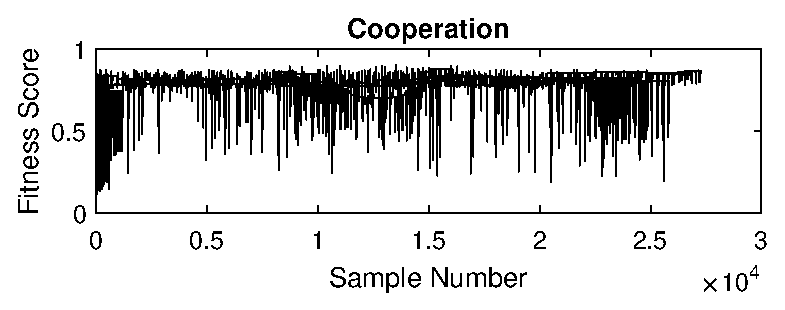
\includegraphics[scale=1]{figures/matlab_sim_results/fitObserved_coop.eps}
\end{subfigure}
\end{center}
\begin{center}
\begin{subfigure}{\linewidth}
	\centering
	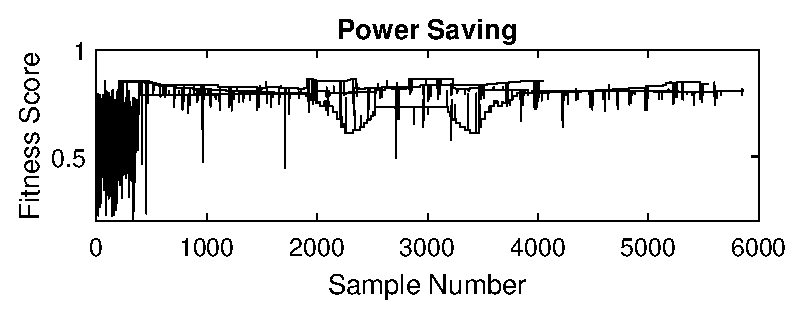
\includegraphics[scale=1]{figures/matlab_sim_results/fitObserved_powerSave.eps}
\end{subfigure}
\end{center}
\caption{Fitness score plotted over length of simulation.}\label{res:matSimFitscore}
\end{figure}
\par A few things are evident with the time series plots shown in \ref{res:matSimFitscore}. The first is that the spurs that are periodically showing up are the CE exploring random actions, and are spaced in a manner independent of training type. In addition, it is apparent that some mission types have different ranges of fitness scores that are possible within the action space, as the cooperation simulation has explorations that have a wider range of values than either the emergency simulation or the power saving simulation. Beyond this, it is evident that LM has a more difficult time than the other two training algorithms in adapting to the higher SNR portions of the simulated pass in both the cooperation and powersaving mission cases. Beyond this, it's fairly difficult to draw conclusions from these time series plots.
\begin{figure}
\centering
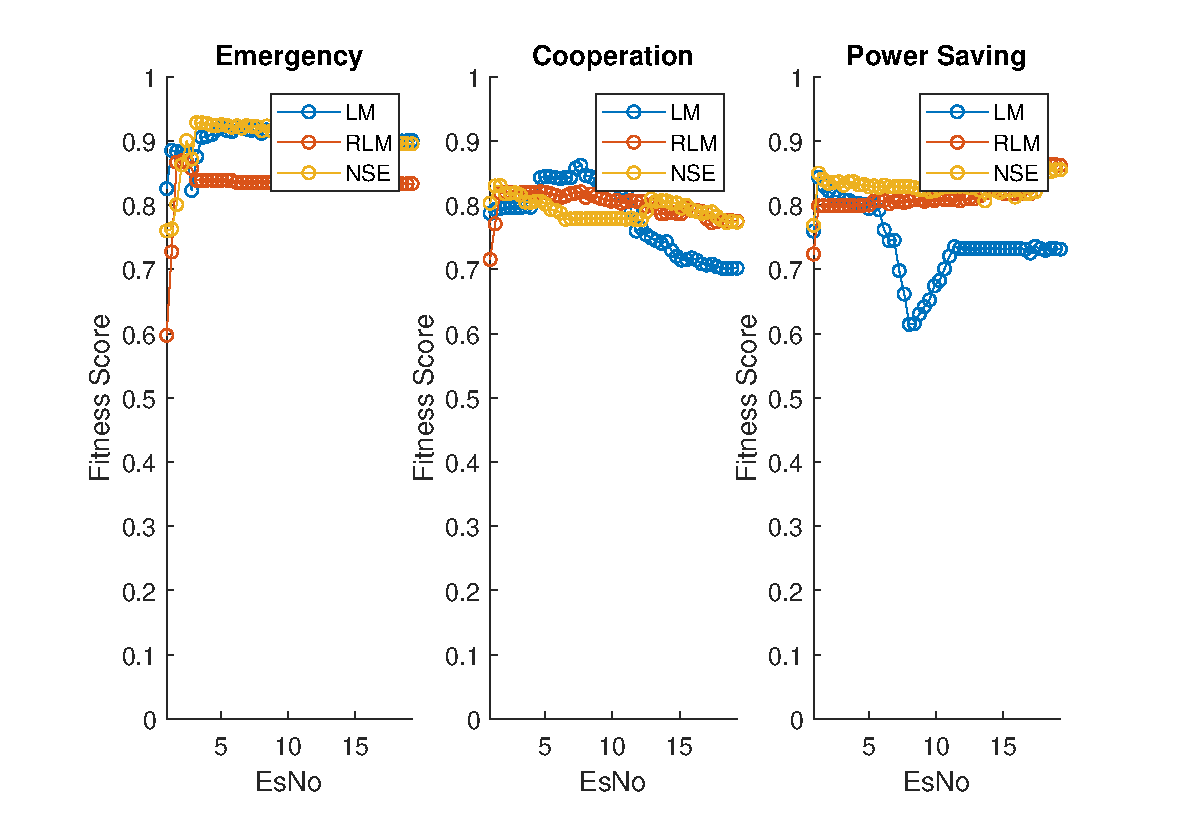
\includegraphics[width=\textwidth]{figures/matlab_sim_results/binnedMeans_sim.eps}
\caption{Value taking the mean fitness value}
\label{res:matSimBinMean}
\end{figure}
\par In order to get a better understanding of the behavior of the different modifications of the CE, fitness scores were split into bins based on the EsNo at the moment that the fitness was observed. Once this was done, the mean was taken within each bin. This plot is shown in Figure \ref{res:matSimBinMean}. For the Emergency mission, LM and NSE proved to have similar average fitness scores, with RLM having lower average fitness scores. The cooperation mission was more ambiguous, with RLM and NSE performing better than LM in the higher EsNo regime, and performing worse than LM in the middle EsNo regime. Finally, the power saving mission shows both LM and RLM working markedly better than LM in the entire regime.
\par With the results shown in this section, there was enough motivation to progress from the MATLAB simulation to simulation, ground testing, and flight testing in C++. 
% \newpage
\clearpage
\section{Simulation results, C++}
\par Simulations using the C++ implementation of the CE served two main purposes. The first purpose of C++ simulations was to verify the correct operation of the code. The second purpose is to provide a completely identical EsNo profile with which to compare the different training algorithms. As much as the NASA flight staff intended to use useful and consistent metrics when evaluating the quality of the communications channel during the window of opportunity when the ISS can be communicated with, the variation of conditions within each quality category resulted in the different tests conducted between 2017 and 2018 having pass qualities that were \textit{fairly\textbf{[this word is probably too vague]}} different from each other, making them harder to directly compare. Running a simulation allows for more direct comparison, albeit without the possibility of shifting the action space in a way that breaks the communication link.
\par The SNR profiles used in the C++ simulation come from attenuation profiles that were measured by NASA employees at GRC. These profiles are used with variable attenuators to simulate channel conditions. By subtracting these values from the maximum EsNo that the CE is expected to see, the attenuation. These values were fed to the CE. One example pass is shown in Figure \ref{result:cSimSNRProfile}, while the rest can be found in Appendix \ref{app:cSNRProfiles_all}. 
\begin{figure}
\section{Ground Test and Integration}
\begin{itemize}
	\item \textbf{\textit{[DISCUSS PRETRAINING]}}
	\item Time series plot.
	\item histogram
	\item rel histogram
	\item 2d hist, rel, log
	\item binned mean
	\item binned median
	\item sum of binned means and binned medians.
	\item Entire work in appendix.
\end{itemize}

\section{Flight Test results}

\begin{itemize}
	\item \textbf{\textit{[DISCUSS PRETRAINING]}}
	\item Time series plot.
	\item histogram
	\item rel histogram
	\item 2d hist, rel, log
	\item binned mean
	\item binned median
	\item sum of binned means and binned medians.
	\item Entire work in appendix.
\end{itemize}
	\chapter{Conclusion and Future Work} \label{ch:conclusion}

\section{intro to conclusion}
\par In this thesis, the cognitive engine developed for space communications was modified to address the problem of Catastrophic Forgetting. After testing and implementation, the modifications proved to improve performance of the CE. In the following section, the salient achievements of the thesis are described and potential future work is provided.

\section{Research Achievements}
\par Based on the current state-of-the-art and the work conducted by \cite{paulo_theory_paper} and \cite{tim_implementation_paper}, there were two main extensions provided by this thesis:
\begin{itemize}
	\item \textbf{CE-NSE mitigated some effects of Catastrophic Forgetting, and outperformed the baseline CE:} Cognitive engines for autonomous space communications that address Catastrophic Forgetting were developed and tested onboard the ISS. The performance of both CE-RLM and CE-NSE were compared to the baseline CE-LM implementation tested in \cite{tim_implementation_paper}. CE-NSE proved to provide modest improvements in actions chosen without imposing an unreasonble training time penalty.

	\item \textbf{GANs were determined to not be directly applicable to the CE architecture: } The concept of two networks collaboratively working together was present in both the CE and GANs. However, the low supply of offline training data for the GAN makes it unlikely that any GAN employed would be trained sufficiently to have converged on the proper data distribution. In addition, the GAN would likely have to be supplementary to the RLNN structure, instead of replacing the Explore and Exploit networks. 
\end{itemize}

\section{Future Work}
\begin{itemize}
\item One of the goals that did not have time to be completed was the extension of the CE to MAC layer parameters.  Adding this layer greatly increases the action space possible and the evaluation metrics that must be balanced. Integrating this aspect was deemed too complex for this thesis, but could provide significant imporvements.
\item The implementation of CE-NSE simply prunes the ensemble of MLPs by getting rid of the oldest one, under the assumption that the oldest MLP will be the least relevant to the current set of data. This assumption is not necessarily correct. Using a smarter pruning method could continue to improve the results of the CE.
\item CE-NSE uses MSE when evaluating the performance of the individual MLPs in the ensemble. This may not be the best way to evaluate the performance of the MLPs. Instead, a metric more relevant to Satellite Communications may be more relevant.
\item Pretraining was conducted using a small subset of SNR profiles, in the simplest manner possible. A more prinicipled building of an ensemble (such as training individual networks on different portions of an SNR profile that are common) could provide additional improvements.

	
	
\chapter{Appendix}

\par Here are the appendices go.
	
	% Bibliography
	\singlespacing
	\nocite{*}
	\bibliographystyle{unsrt}
	\bibliography{7_references}
	
\end{document}
